\bta{$ 2018 $ 年全国普通高等学校招生考试(全国卷 \lmd{1} ) }

\begin{center}
\heiti 
\zihao{4}
物理部分
\end{center}
\vspace{2em}



\begin{enumerate}
\heiti
\renewcommand{\labelenumi}{\arabic{enumi}.}
% A(\Alph) a(\alph) I(\Roman) i(\roman) 1(\arabic)
%设定全局标号series=example	%引用全局变量resume=example
%[topsep=-0.3em,parsep=-0.3em,itemsep=-0.3em,partopsep=-0.3em]
%可使用leftmargin调整列表环境左边的空白长度 [leftmargin=0em]
\item[一、]
选择题:本题共 $ 8 $ 小题,每小题 $ 6 $ 分。在每小题给出的四个选项中,第 $ 1 \sim 5 $ 题只有一项符合题
目要求,第 $ 6 \sim 8 $ 题有多项符合题目要求。全部选对的得 $ 6 $ 分,选对但不全的得 $ 3 $ 分,有选错的
得 $ 0 $ 分。




\end{enumerate}


\begin{enumerate}
\renewcommand{\labelenumi}{\arabic{enumi}.}
% A(\Alph) a(\alph) I(\Roman) i(\roman) 1(\arabic)
%设定全局标号series=example	%引用全局变量resume=example
%[topsep=-0.3em,parsep=-0.3em,itemsep=-0.3em,partopsep=-0.3em]
%可使用leftmargin调整列表环境左边的空白长度 [leftmargin=0em]
\item
高铁列车在启动阶段的运动可看作初速度为零的匀加速直线运动,在启动阶段,列车的动能 \xzanswer{B} 

\fourchoices
{与它所经历的时间成正比}
{与它的位移成正比}
{与它的速度成正比}
{与它的动量成正比}


\item
如图,轻弹簧的下端固定在水平桌面上,上端放有物块 $ P $,系统处于静止状态,现用一竖直向
上的力 $ F $ 作用在 $ P $ 上,使其向上做匀加速直线运动,以 $ x $ 表示 $ P $ 离开静止位置的位移,在弹
簧恢复原长前,下列表示 $ F $ 和 $ x $ 之间关系的图像可能正确的是 \xzanswer{A} 

\begin{figure}[h!]
\centering
\includesvg[width=0.63\linewidth]{picture/svg/921}
\end{figure}




\item
如图,三个固定的带电小球 $ a $ 、$ b $ 和 $ c $ ,相互间的距离分别为 $ ab=5 \ cm $,$ bc=3 \ cm $,$ ca=4 \ cm $。
小球 $ c $ 所受库仑力的合力的方向平行于 $ a $ 、 $ b $ 的连线。设小球 $ a $ 、 $ b $ 所带电荷量的比值的绝对
值为 $ k $ ,则 \xzanswer{D} 

\begin{figure}[h!]
\centering
\includesvg[width=0.43\linewidth]{picture/svg/922}
\end{figure}

\fourchoices
{$ a $ 、 $ b $ 的电荷同号, $k=\frac{16}{9}$}
{$ a $ 、 $ b $ 的电荷异号, $k=\frac{16}{9}$}
{$ a $ 、 $ b $ 的电荷同号, $k=\frac{64}{27}$}
{$ a $ 、 $ b $ 的电荷异号, $k=\frac{64}{27}$}



\banswer{

}

\item
如图,导体轨道 $ OPQS $ 固定,其中 $ PQS $ 是半圆弧,$ Q $ 为半圆弧的中点,$ O $ 为圆心。轨道的电阻
忽略不计。$ OM $ 是有一定电阻。可绕 $ O $ 转动的金属杆。$ M $ 端位于 $ PQS $ 上,$ OM $ 与轨道接触良
好。空间存在与半圆所在平面垂直的匀强磁场,磁感应强度的大小为 $ B $,现使 $ OM $ 从 $ OQ $ 位置
以恒定的角速度逆时针转到 $ OS $ 位置并固定(过程$ \lmd{1} $);再使磁感应强度的大小以一定的变化
率从 $ B $ 增加到 $ B ^{\prime} $(过程$ \lmd{2} $)。在过程$ \lmd{1} $、$ \lmd{2} $中,流过 $ OM $ 的电荷量相等,则$\frac{B^{\prime}}{B}$等于 \xzanswer{B} 

\begin{figure}[h!]
\centering
\includesvg[width=0.23\linewidth]{picture/svg/923}
\end{figure}


\fourchoices
{$ \frac{ 5 }{ 4 } $}
{$ \frac{ 3 }{ 2 } $}
{$ \frac{ 7 }{ 4 } $}
{$ 2 $}


\banswer{

}


\newpage
\item
如图, $ abc $ 是竖直面内的光滑固定轨道, $ ab $ 水平,长度为 $ 2R $; $ bc $ 是半径为 $ R $ 的四分之一的圆
弧,与 $ ab $ 相切于 $ b $ 点。一质量为 $ m $ 的小球。始终受到与重力大小相等的水平外力的作用,自
$ a $ 点处从静止开始向右运动,重力加速度大小为 $ g $。小球从 $ a $ 点开始运动到其轨迹最高点,机
械能的增量为 \xzanswer{C} 

\begin{figure}[h!]
\centering
\includesvg[width=0.38\linewidth]{picture/svg/924}
\end{figure}

\fourchoices
{$ 2 mgR $}
{$ 4 mgR $}
{$ 5 mgR $}
{$ 6 mgR $}


\banswer{

}

\item
如图,两个线圈绕在同一根铁芯上,其中一线圈通过开关与电源连接,另一线圈与远处沿南北方向水平
放置在纸面内的直导线连接成回路。将一小磁针悬挂在直导线正上方,开关未闭合时小磁针处于静止
状态。下列说法正确的是 \xzanswer{AD} 

\begin{figure}[h!]
\centering
\includesvg[width=0.23\linewidth]{picture/svg/925}
\end{figure}

\fourchoices
{开关闭合后的瞬间,小磁针的 $ N $ 极朝垂直纸面向里的方向转动}
{开关闭合并保持一段时间后,小磁针的 $ N $ 极指向垂直纸面向里的方向}
{开关闭合并保持一段时间后,小磁针的 $ N $ 极指向垂直纸面向外的方向}
{开关闭合并保持一段时间再断开后的瞬间,小磁针的 $ N $ 极朝垂直纸面向外的方向转动}

\banswer{

}


\newpage

\item 
$ 2017 $ 年,人类第一次直接探测到来自双中子星合并的引力波。根据科学家们复原的过程,在两
颗中子星合并前约 $ 100 \ s $ 时,它们相距约 $ 400 \ km $,绕二者连线上的某点每秒转动 $ 12 $ 圈,将两
颗中子星都看作是质量均匀分布的球体,由这些数据、万有引力常量并利用牛顿力学知识,可
以估算出这一时刻两颗中子星 \xzanswer{BC} 


\fourchoices
{质量之积}
{质量之和}
{速率之和}
{各自的自转角速度}

\banswer{

}


\item
图中虚线 $ a $ 、 $ b $ 、 $ c $ 、 $ d $ 、 $ f $ 代表匀强电场内间距相等的一组等势面,已知平面 $ b $ 上的电势为 $ 2 $
$ V $。一电子经过 $ a $ 时的动能为 $ 10 \ eV $,从 $ a $ 到 $ d $ 的过程中克服电场力所做的功为 $ 6 \ eV $。下列说
法正确的是 \xzanswer{AB} 

\begin{figure}[h!]
\centering
\includesvg[width=0.33\linewidth]{picture/svg/926}
\end{figure}

\fourchoices
{平面 $ c $ 上的电势为零}
{该电子可能到达不了平面 $ f $}
{该电子经过平面 $ d $ 时,其电势能为 $ 4 \ eV $}
{该电子经过平面 $ b $ 时的速率是经过 $ d $ 时的 $ 2 $ 倍}

\banswer{

}


\newpage
\begin{enumerate}[leftmargin=-2em]
\renewcommand{\labelenumii}{}
% A(\Alph) a(\alph) I(\Roman) i(\roman) 1(\arabic)
%可使用leftmargin调整列表环境左边的空白长度
\item
\btd{二、非选择题}
\btd{(一)必考题}
\end{enumerate}


\item
($ 5 $ 分)如图($ a $),一弹簧上端固定在支架顶端,下端悬挂一托盘:一标尺由游标和主尺构成,
主尺竖直固定在弹簧左边;托盘上方固定有一能与游标刻度线准确对齐的装置,简化为图中的
指针。

现要测量图($ a $)中弹簧的劲度系数,当托盘内没有砝码时,移动游标,使其零刻度线对
准指针,此时标尺读数为 $ 1.950 \ cm $;当托盘内放有质量为 $ 0.100 \ kg $ 的砝码时,移动游标,再
次使其零刻度线对准指针,标尺示数如图($ b $)所示,其读数为 \tk{$ 3.775 $} $ cm $。当地的重力加速度大
小为 $ 9.80 \ m/s^{2} $,此弹簧的劲度系数为 \tk{$ 53.7 $} $ N/m $(保留 $ 3 $ 位有效数字)。
\begin{figure}[h!]
\centering
\includesvg[width=0.37\linewidth]{picture/svg/927}
\end{figure}


\newpage

\item 
($ 10 $ 分)某实验小组利用如图($ a $)所示的电路探究在 $ 25 \ \celsius \sim 80 \ \celsius $范围内某热敏电阻的温度特
性,所用器材有:置于温控室(图中虚线区域)中的热敏电阻 $ R_T $ ,其标称值($ 25 \ \celsius $时的阻值)
为 $ 900.0 \ \Omega $:电源 $ E $($ 6 \ V $,内阻可忽略):电压表
\voltmetermytikz 
(量程 $ 150 \ mV $):定值电阻 $ R_{0} $ (阻值 $ 20.0 \ \Omega $),滑动变阻器 $ R_{1} $(最大阻值为 $ 1000 \ \Omega $):电阻箱 $ R_{2} $ (阻值范围 $ 0-999.9 \ \Omega $):单刀开关 $ S_{1} $ ,
单刀双掷开关 $ S_{2} $ 。
\begin{figure}[h!]
\centering
\includesvg[width=0.43\linewidth]{picture/svg/928}
\end{figure}



实验时,先按图($ a $)连接好电路,再将温控室的温度 $ t $ 升至 $ 80.0 \ \celsius $,将 $ S_{2} $ 与 $ 1 $ 端接通,闭合 $ S_{1} $,
调节 $ R_{1} $ 的滑片位置,使电压表读数为某一值 $ U_{0} $ :保持 $ R_{1} $ 的滑片位置不变,将 $ R_{2} $ 置于最大值,
将 $ S_{2} $ 与 $ 2 $ 端接通,调节 $ R_{2} $ ,使电压表读数仍为 $ U_{0} $ :断开 $ S_{1} $ ,记下此时 $ R_{2} $ 的读数,逐步降低
温控室的温度 $ t $ ,得到相应温度下 $ R_{2} $ 的阻值,直至温度降到 $ 25.0 ^{ \circ } C $,实验得到的 $ R_{2} -t $ 数据见
下表。

\begin{table}[h!]
\centering 
\begin{tabular}{|c|c|c|c|c|c|c|c|}
\hline 
$ t/ \celsius $ & 25.0 & 30.0 & 40.0 & 50.0 & 60.0 & 70.0 & 80.0
\\
\hline
$ R_2/ \Omega $ & 900.0 & 680.0 & 500.0 & 390.0 & 320.0 & 270.0 & 240.0\\ 
\hline 
\end{tabular}
\end{table} 


回答下列问题:
\begin{enumerate}
\renewcommand{\labelenumi}{\arabic{enumi}.}
% A(\Alph) a(\alph) I(\Roman) i(\roman) 1(\arabic)
%设定全局标号series=example	%引用全局变量resume=example
%[topsep=-0.3em,parsep=-0.3em,itemsep=-0.3em,partopsep=-0.3em]
%可使用leftmargin调整列表环境左边的空白长度 [leftmargin=0em]
\item
在闭合 $ S_{1} $ 前,图($ a $)中 $ R_{1} $ 的滑片应移动到
\tk{$ b $} 
(填“$ a $”或“$ b $”)端;




\item 
在图($ b $)的坐标纸上补齐数据表中所给数据点,并做出 $ R_{2} -t $ 曲线:
\begin{figure}[h!]
\centering
\includesvg[width=0.73\linewidth]{picture/svg/929}
\end{figure}

%答案
%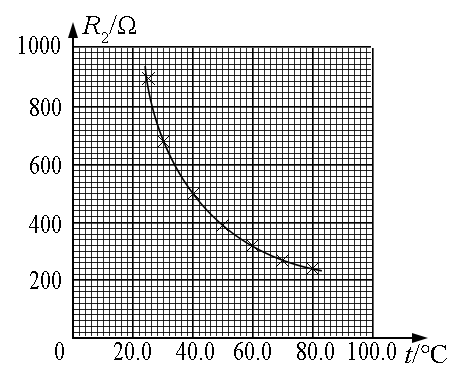
\includegraphics[width=0.7\linewidth]{picture/screenshot021}


\item 
由图($ b $)可得到 $ R_T $ 在 $ 25 \ \celsius -80 ^{ \circ } C $ 范围内的温度特性,当 $ t=44.0 \ \celsius $时,
可得 $ R_T= $
\tk{$ 450 $} 
$ \Omega $;




\item 
将 $ R_T $ 握于手心,手心温度下 $ R_{2} $ 的相应读数如图($ c $)所示,该读数为
为
\tk{$ 620.0 $} 
$ \Omega $,则手心温度
\tk{$ 33.0 $} 
$ \celsius $。




\end{enumerate}



\banswer{

}



\item 
($ 12 $ 分)一质量为 $ m $ 的烟花弹获得动能 $ E $ 后,从地面竖直升空,当烟花弹上升的速度为零时,
弹中火药爆炸将烟花弹炸为质量相等的两部分,两部分获得的动能之和也为 $ E $ ,且均沿竖直方
向运动。爆炸时间极短,重力加速度大小为 $ g $,不计空气阻力和火药的质量,求:
\begin{enumerate}
\renewcommand{\labelenumi}{\arabic{enumi}.}
% A(\Alph) a(\alph) I(\Roman) i(\roman) 1(\arabic)
%设定全局标号series=example	%引用全局变量resume=example
%[topsep=-0.3em,parsep=-0.3em,itemsep=-0.3em,partopsep=-0.3em]
%可使用leftmargin调整列表环境左边的空白长度 [leftmargin=0em]
\item
烟花弹从地面开始上升到弹中火药爆炸所经过的时间;



\item 
爆炸后烟花弹向上运动的部分距地面的最大高度。




\end{enumerate}

\banswer{
\begin{enumerate}
\renewcommand{\labelenumi}{\arabic{enumi}.}
% A(\Alph) a(\alph) I(\Roman) i(\roman) 1(\arabic)
%设定全局标号series=example	%引用全局变量resume=example
%[topsep=-0.3em,parsep=-0.3em,itemsep=-0.3em,partopsep=-0.3em]
%可使用leftmargin调整列表环境左边的空白长度 [leftmargin=0em]
\item
$t=\frac{1}{g} \sqrt{\frac{2 E}{m}}$
\item 
$h=h_{1}+h_{2}=\frac{2 E}{m g}$

\end{enumerate}


}

\newpage

\item 
($ 20 $ 分)如图,在 $ y>0 $ 的区域存在方向沿 $ y $ 轴负方向的匀强电场,场强大小为 $ E $ ,在 $ y<0 $
的区域存在方向垂直于 $ xOy $ 平面向外的匀强磁场。一个氕核 $ ^{1}_{1}H $ 和一个氘核 $ ^{2}_{1}H $ 先后从 $ y $ 轴上
$ y=h $ 点以相同的动能射出,速度方向沿 $ x $ 轴正方向。已知 $ ^{1}_{1}H $ 进入磁场时,速度方向与 $ x $ 轴
正方向的夹角为 $ 60 ^{ \circ } $,并从坐标原点 $ O $ 处第一次射出磁场。 $ ^{1}_{1}H $ 的质量为 $ m $ ,电荷量为 $ q $ 。不
计重力。求:
\begin{enumerate}
\renewcommand{\labelenumi}{\arabic{enumi}.}
% A(\Alph) a(\alph) I(\Roman) i(\roman) 1(\arabic)
%设定全局标号series=example	%引用全局变量resume=example
%[topsep=-0.3em,parsep=-0.3em,itemsep=-0.3em,partopsep=-0.3em]
%可使用leftmargin调整列表环境左边的空白长度 [leftmargin=0em]
\item
$ ^{1}_{1}H $ 第一次进入磁场的位置到原点 $ O $ 的距离;



\item 
磁场的磁感应强度大小;





\item 
$ ^{2}_{1}H $ 第一次离开磁场的位置到原点 $ O $ 的距离。




\end{enumerate}
\begin{figure}[h!]
\flushright
\includesvg[width=0.25\linewidth]{picture/svg/930}
\end{figure}

\banswer{
\begin{enumerate}
\renewcommand{\labelenumi}{\arabic{enumi}.}
% A(\Alph) a(\alph) I(\Roman) i(\roman) 1(\arabic)
%设定全局标号series=example	%引用全局变量resume=example
%[topsep=-0.3em,parsep=-0.3em,itemsep=-0.3em,partopsep=-0.3em]
%可使用leftmargin调整列表环境左边的空白长度 [leftmargin=0em]
\item
$s_{1}=\frac{2 \sqrt{3}}{3} h$
\item 
$B=\sqrt{\frac{6 m E}{q h}}$
\item 
$s_{2}^{\prime}-s_{2}=\frac{2 \sqrt{3}}{3}(\sqrt{2}-1) h$
\end{enumerate}


}




\begin{enumerate}[leftmargin=-2em]
\renewcommand{\labelenumii}{}
% A(\Alph) a(\alph) I(\Roman) i(\roman) 1(\arabic)
%可使用leftmargin调整列表环境左边的空白长度
\item
\btd{(二)选考题}
\end{enumerate}


\item 

[物理—选修 $ 3-3 $]($ 15 $ 分)


\begin{enumerate}
\renewcommand{\labelenumi}{\arabic{enumi}.}
% A(\Alph) a(\alph) I(\Roman) i(\roman) 1(\arabic)
%设定全局标号series=example	%引用全局变量resume=example
%[topsep=-0.3em,parsep=-0.3em,itemsep=-0.3em,partopsep=-0.3em]
%可使用leftmargin调整列表环境左边的空白长度 [leftmargin=0em]
\item
($ 5 $ 分)如图,一定质量的理想气体从状态 $ a $ 开始,经历过程①、②、③、④到达状态 $ e $ ,
对此气体,下列说法正确的是
\tk{BDE} 
(选对 $ 1 $ 个得 $ 2 $ 分,选对 $ 2 $ 个得 $ 4 $ 分,选对 $ 3 $ 个得 $ 5 $
分:每选错 $ 1 $ 个扣 $ 3 $ 分,最低得分为 $ 0 $ 分)。
\begin{figure}[h!]
\centering 
\includesvg[width=0.3\linewidth]{picture/svg/931}
\end{figure}



\fivechoices
{过程①中气体的压强逐渐减小}
{过程②中气体对外界做正功}
{过程④中气体从外界吸收了热量}
{状态 $ c $ 、 $ d $ 的内能相等}
{状态 $ d $ 的压强比状态 $ b $ 的压强小}



\item 
($ 10 $ 分)如图,容积为 $ V $ 的汽缸由导热材料制成,面积为 $ S $ 的活塞将汽缸分成容积相等的
上下两部分,汽缸上部通过细管与装有某种液体的容器相连,细管上有一阀门 $ K $ 。开始
时, $ K $ 关闭,汽缸内上下两部分气体的压强均为 $ p_{0} $ .现将 $ K $ 打开,容器内的液体缓慢
地流入汽缸,当流入的液体体积为
$ \frac{V}{8} $
时,将 $ K $ 关闭,活塞平衡时其下方气体的体积减小了$ \frac{V}{6} $,不计活塞的质量和体积,外界温度保持不变,重力加速度大小为 $ g $。求流入汽缸
内液体的质量。
\begin{figure}[h!]
\flushright
\includesvg[width=0.25\linewidth]{picture/svg/932}
\end{figure}


\banswer{
$m=\frac{15 p_{0} S}{26 g}$	
}


\end{enumerate}




\newpage
\item 

[物理一选修 $ 3-4 $)($ 15 $ 分)


\begin{enumerate}
\renewcommand{\labelenumi}{\arabic{enumi}.}
% A(\Alph) a(\alph) I(\Roman) i(\roman) 1(\arabic)
%设定全局标号series=example	%引用全局变量resume=example
%[topsep=-0.3em,parsep=-0.3em,itemsep=-0.3em,partopsep=-0.3em]
%可使用leftmargin调整列表环境左边的空白长度 [leftmargin=0em]
\item
($ 5 $ 分)如图, $ \triangle ABC $ 为一玻璃三棱镜的横截面, $ \angle A=30 ^{\circ} $ ,一束红光垂直 $ AB $ 边射入,
从 $ AC $ 边上的 $ D $ 点射出,其折射角为 $ 60 ^{\circ} $ ,则玻璃对红光的折射率为 \tk{$\sqrt{3}$} 。若改用蓝光
沿同一路径入射,则光线在 $ D $ 点射出时的折射角 \tk{大于} (“小于”“等于”或“大于”) $ 60 ^{\circ} $ 。
\begin{figure}[h!]
\centering
\includesvg[width=0.43\linewidth]{picture/svg/933}
\end{figure}




\item 
($ 10 $ 分)一列简谐横波在 $ t= \frac{ 1 }{ 3 } s $ 时的波形图如图($ a $)所示,$ P $、$ Q $ 是介质中的两个质点,
图($ b $)是质点 $ Q $ 的振动图像。求:
\begin{enumerate}
\renewcommand{\labelenumiii}{\roman{enumiii}.}
% A(\Alph) a(\alph) I(\Roman) i(\roman) 1(\arabic)
%设定全局标号series=example	%引用全局变量resume=example
%[topsep=-0.3em,parsep=-0.3em,itemsep=-0.3em,partopsep=-0.3em]
%可使用leftmargin调整列表环境左边的空白长度 [leftmargin=0em]
\item
波速及波的传播方向;
\item 
质点 $ Q $ 的平衡位置的 $ x $ 坐标。




\end{enumerate}
\begin{figure}[h!]
\flushright
\includesvg[width=0.55\linewidth]{picture/svg/934}
\end{figure}


\banswer{
\begin{enumerate}
\renewcommand{\labelenumi}{\arabic{enumi}.}
% A(\Alph) a(\alph) I(\Roman) i(\roman) 1(\arabic)
%设定全局标号series=example	%引用全局变量resume=example
%[topsep=-0.3em,parsep=-0.3em,itemsep=-0.3em,partopsep=-0.3em]
%可使用leftmargin调整列表环境左边的空白长度 [leftmargin=0em]
\item
波沿负方向传播
\item 
$x_{Q}=9\ \mathrm{cm}$

\end{enumerate}


}



\end{enumerate}



\end{enumerate}


